\begin{figure}
    \centering
    \resizebox{0.48\textwidth}{!}{%
        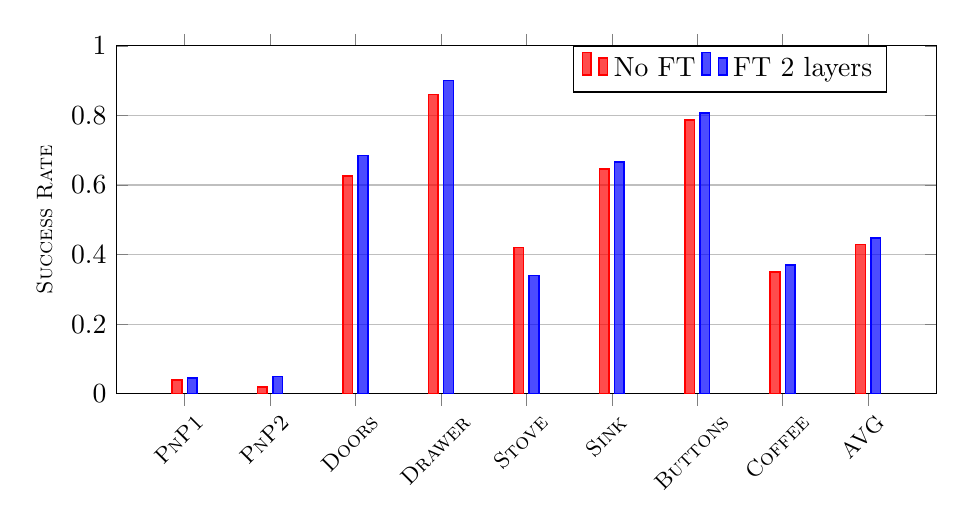
\begin{tikzpicture}[baseline]
        % \definecolor{red}{RGB}{214,39,40}
        % \definecolor{blue}{RGB}{31,119,180}
        
        \begin{axis}[
            ybar,
            height=6cm, width=12cm,
            bar width=3.5pt,
            ylabel=Success Rate,
            ylabel style={
                font=\footnotesize\scshape
            },
            ymin=0, ymax=1,
            legend style={at={(0.748, 1)}, anchor=north, legend columns=-1},
            symbolic x coords={PnP1, PnP2, Doors, Drawer, Stove, Sink, Buttons, Coffee, AVG},
            xtick=data,
            xticklabel style={
                rotate=45,
                font=\footnotesize\scshape,
                yshift=3pt,
            },
            ymajorgrids
        ]
        
        \addplot [
            draw=red,
            fill=red,
            line width=.2mm,
            fill opacity=0.7
        ] coordinates {
            (PnP1, 0.0400)
            (PnP2, 0.0200)
            (Doors, 0.6250)
            (Drawer, 0.8600)
            (Stove, 0.4200)
            (Sink, 0.6467)
            (Buttons, 0.7867)
            (Coffee, 0.3500)
            (AVG, 0.4292)
        };

        \addplot [
            draw=blue,
            fill=blue,
            line width=.2mm,
            fill opacity=0.7
        ] coordinates {
            (PnP1, 0.0450)
            (PnP2, 0.0500)
            (Doors, 0.6850)
            (Drawer, 0.9000)
            (Stove, 0.3400)
            (Sink, 0.6667)
            (Buttons, 0.8067)
            (Coffee, 0.3700)
            (AVG, 0.4483)
        };

        \legend{No FT, FT 2 layers}
        \end{axis}
        
        \end{tikzpicture}
    }
    \caption{Success rates using different finetuning strategies for the pretrained SUGAR encoder.}
    \vspace{-10pt} 
    \label{fig:ablation_sugar_ft}
\end{figure}
